\icode{E-MM-SI-L3-261013-002}
如图所示为一种基于伽利略大炮原理的简易模型，两小球 \(P\)、\(Q\) 竖直叠放在一起，小球间留有较小空隙，从距水平地面高度为 \(h\) 处同时由静止释放。已知小球 \(Q\) 的质量是 \(P\) 的 3 倍。设所有碰撞均为弹性碰撞，忽略空气阻力及碰撞时间，则两球第一次碰撞后小球 \(P\) 上升的高度为\paren[]

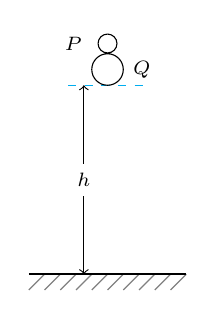
\begin{tikzpicture}[font=\scriptsize]
	\foreach \x in {-1,-.8,...,.8}
		\draw[gray] (\x,-.2)--++(.2,.2);
	\draw[thick] (-1,0)--(1,0);
	\draw[dashed,cyan] (-.5,2.4)--(.5,2.4);
	\draw[<->,thin] (-.3,0)--node[fill=white]{\(h\)}(-.3,2.4);
	\draw[fill=white] (0,2.6) circle(.2) (0,2.93) circle(.12);
	\node at(.2,2.6)[right]{\(Q\)};
	\node at(-.2,2.93)[left]{\(P\)};
\end{tikzpicture}
\begin{choices}
	\item \(\frac{5}{3}h\)
	\item \(\frac{25}{9}h\)
	\item \(4h\)
	\item \(5h\)
\end{choices}
\begin{answer}
    C\qquad 提示：\(v_1^{\prime} = \frac{(m_1 - m_2)v_1 + 2m_2v_2}{m_1 + m_2}\)\quad \(v_2^{\prime} = \frac{(m_2 - m_1)v_2 + 2m_1v_1}{m_1 + m_2}\)
\end{answer}